\documentclass[10pt,a4paper]{article}

\usepackage[utf8]{inputenc}		% Configuro la codificación
\input{.command.tex}
% En el siguiente archivo se configuran las variables del trabajo práctico
%% \providecommand es similar a \newcommnad, salvo que el primero ante un 
%% conflicto en la compilación, es ignorado.

% Al comienzo de un TP se debe modificar los argumentos de los comandos

\providecommand{\myTitle}{ACTIVIDAD 3}
\providecommand{\mySubtitle}{Fuentes conmutadas}

\providecommand{\mySubject}{Diseño de Circuitos Electrónicos (86.10)}
\providecommand{\myKeywords}{UBA, Ingeniería, C2}

\providecommand{\myAuthorSurname}{Alonso, Manso, Zuccolo}
\providecommand{\myTimePeriod}{Año 2018 - 2\textsuperscript{do} Cuatrimestre}

% No es necesario modificar este %%%%%%%%%%%%%%
\providecommand{\myHeaderLogo}{header_fiuba}
%%%%%%%%%%%%%%%%%%%%%%%%%%%%%%%%%%%%%%%%%%%%%%%%

% Si se utilizan listings, definir el lenguaje aquí
\providecommand{\myLanguage}{matlab}

% Crear los integrantes del TP con el comando \PutMember donde
%%		1) Apellido, Nombre
%%		2) Número de Padrón
%%		3) E-Mail
\providecommand{\MembersOnCover}[0]
{		
		\PutMember{Alonso, Gustavo Gabriel} {96119} {gustavoalon19@gmail.com}
		\PutMember{Manso, Juan} {96133} {juanmanso@gmail.com}
		\PutMember{Russo, Nicolas Emanuel} {93211} {nicolasrusso291@gmail.com}
		\PutMember{Zuccolo, Florencia} {96628} {florenciaz618@gmail.com}
}

\providecommand{\myGroupNumber}{10}

\Pagebreaktrue		% Setea si hay un salto de página en la carátula
\Indextrue
\Siunitxtrue			% Si quiero utilizar el paquete, \siunixtrue. Si no \siunixfalse
\Todonotestrue		% Habilita/Deshabilita las To-Do Notes y las funciones \unsure, \change, \info, \improvement y \thiswillnotshow.
\Listingsfalse
\Keywordsfalse
\Putgrouptrue		% Habilita/Deshabilita el \myGroup en los headers
\Videofalse
				% Archivo con los comandos globales como Título y autores
%Preambulo para articulo científico de LaTeX

\usepackage[a4paper,left=3cm,right=3cm,bottom=3.5cm,top=3.5cm]{geometry} 	% Configuro la geometría del papel
%\usepackage{microtype}								% Mejora el "spacing" de las palabras
\usepackage[spanish]{babel} 							% Compatibilizo los signos del español
	\addto\captionsspanish{\renewcommand{\tablename}{Tabla}}		%% Redefino nombres preestablecidos por Babel
	\addto\captionsspanish{\renewcommand{\listtablename}{Índice de tablas}}	%% y así en vez de Cuadro dirá Tabla.
\usepackage{amsmath, amsfonts, amssymb}						% Entornos matemáticos, fuentes y símbolos
\usepackage{graphicx}								% Necesario para insertar figuras
\usepackage{fancyhdr}								% Para manipular headers y footers
\usepackage[usenames,dvipsnames]{color}						% \color{color deseado} {lo que querés que tenga color}
\usepackage{subcaption}								% Permite captions del tipo 1a, 1b
\usepackage{multirow}								% Para tablas
%\usepackage{slashbox}								% Cuadro divido en tablas
\usepackage{diagbox}
\usepackage{float}
\usepackage{multicol}

% Para video
\ifVideo
	\usepackage{media9}
	\addmediapath{./../reportes/}
\fi

%\usepackage{times}
%\usepackage{mathtools}
%\usepackage{upgreek} % letras griegas sin cursiva
%\usepackage{cancel}
\usepackage{rotating}
\usepackage{tikz}
\usepackage{pgfplots}
%	\pgfplotsset{compat=1.12}
	\usetikzlibrary{plotmarks}% matlab2tikz
\usepackage{grffile}% matlab2tikz 
	\usetikzlibrary{calc,patterns,decorations.pathmorphing,decorations.markings}

\ifListings
	\usepackage{listings}

	\providecommand{\lstinputpath}[1]{\lstset{inputpath=#1}}

%	\input{.lst_default.tex}
	\input{.lst_matlab.tex}
%	\input{.lst_c.tex}
%	\input{.lst_c++.tex}
	
% 	\input{.lst_pseudocode.tex}


\fi

\ifSiunitx
\usepackage{siunitx}											% Unidades: \SI {cantidad} {\unidad} (necesita texlive-science)
	\sisetup{load-configurations = abbreviations}							% Habilita poner \cm en vez de \centi\metre
	\sisetup{output-decimal-marker = {,}}									% Cambia los puntos decimales por comas
	\sisetup{per-mode = fraction}											% Pone las unidades como fracción
	\sisetup{quotient-mode = fraction}										
\fi


\ifTodonotes
\usepackage{xargs}
\usepackage[colorinlistoftodos,prependcaption,textsize=tiny]{todonotes}


	\newcommandx{\Juan}[2][1=]{\todo[linecolor=red,backgroundcolor=red!25,bordercolor=red,#1]{#2}}
	\newcommandx{\Flor}[2][1=]{\todo[linecolor=blue,backgroundcolor=blue!25,bordercolor=blue,#1]{#2}}
	\newcommandx{\Gus}[2][1=]{\todo[linecolor=green,backgroundcolor=green!25,bordercolor=green,#1]{#2}} % OliveGreen
	\newcommandx{\Nico}[2][1=]{\todo[linecolor=yellow,backgroundcolor=yellow!25,bordercolor=yellow,#1]{#2}}
	\newcommandx{\thiswillnotshow}[2][1=]{\todo[disable,#1]{#2}}
\fi


\usepackage{booktabs}														% Permite hacer tablas sin separadores en el medio
\usepackage{placeins}														
		\let\Oldsection\section												%% Permite que los flotantes (como figuras) no aparescan
	\renewcommand{\section}{\FloatBarrier\Oldsection}						%% antes o después de su sección correspondiente.
		\let\Oldsubsection\subsection
	\renewcommand{\subsection}{\FloatBarrier\Oldsubsection}		
		\let\Oldsubsubsection\subsubsection
	\renewcommand{\subsubsection}{\FloatBarrier\Oldsubsubsection}
\usepackage{hyperref}														% Debe ser agregado al final del preambulo

\hypersetup
{    bookmarks=true,         % show bookmarks bar?
     unicode=false,          % non-Latin characters in Acrobat’s bookmarks
     pdftoolbar=true,        % show Acrobat’s toolbar?
     pdfmenubar=true,        % show Acrobat’s menu?
     pdffitwindow=false,     % window fit to page when opened
     pdftitle={\myTitle},    		 % title
     pdfauthor={\myAuthorSurname},   % author
	 pdfcreator={\myAuthorSurname},	 % creator = author
     pdfsubject={\mySubject},		 % subject of the document
     pdfkeywords={\myKeywords},
     colorlinks=true,        % false: boxed links; true: colored links
     linkcolor=black,        % color of internal links (change box color with linkbordercolor)
     citecolor=black,        % color of links to bibliography
     filecolor=magenta,      % color of file links
     urlcolor=cyan           % color of external links
}

%Configuro la pagina con los encabezaos y pies de paginas
\pagestyle{fancy}										% Para agregar encabezados y pie de paginas	
%\lhead{\mySubject}										% Encabezado izquierdo
\lhead{DCE (86.10)}
\rhead{\includegraphics[scale=0.15]{\myHeaderLogo}} 	% Encabezado derecho (logo de la FIUBA)	
\ifPutgroup
\chead{\texttt{Grupo Nº\myGroupNumber} \\ \textit{\footnotesize{\myTimePeriod}}}
\fi				

%% Este archivo contiene las funciones auxiliares para escribir en LaTeX
%% Dichas funciones resuelven la sintaxis de generar figuras, por ejemplo,
%% dejando el código más compacto y facilitando la corrección del mismo.



% Comando para graficar eps. 1er arg, escala. 2do, ruta. 3ro, caption. 4to, label.
\providecommand{\HgraficarEPS}[4]{
			\begin{figure}[h!]
				\centering
					\scalebox{#1}{\input{#2}}
					\caption{#3}
					\label{#4}
			\end{figure}

}

\providecommand{\HgraficarPNG}[4]{
			\begin{figure}[h!]
				\centering
					\includegraphics[scale=#1]{#2}
					\caption{#3}
					\label{#4}
			\end{figure}

}


% Comando para graficar eps en el lugar previsto.
\providecommand{\graficarEPS}[4]{
			\begin{figure}[h]
				\centering
					\scalebox{#1}{\input{#2}}
					\caption{#3}
					\label{#4}
			\end{figure}

}

\providecommand{\graficarPNG}[4]{
			\begin{figure}[h]
				\centering
					\includegraphics[scale=#1]{#2}
					\caption{#3}
					\label{#4}
			\end{figure}

}

\providecommand{\underuparrow}[2]{\underset{\underset{#2} \uparrow} #1 }

\providecommand{\cltext}[2]{\color{#1}{\huge{#2}}}
\providecommand{\cstext}[2]{\color{#1}{\large{#2}}}

\providecommand{\lsi}[1]{\large\si{#1}}
\providecommand{\lsio}[0]{\large\si{\ohm}}
\providecommand{\lsiv}[0]{\large\si{\volt}}
\providecommand{\lsia}[0]{\large\si{\ampere}}
\providecommand{\lSI}[2]{\large\SI{#1}{#2}}


		% Se proveen un conjunto de funciones extras

% Defino el path de los includegraphics
\graphicspath{{./Figuras/}}		% Directorio que contiene los graficos

% Defino el path para los input de .tex y de .eps
\makeatletter
\def\input@path{{./Figuras/}{./Secciones/}{./Cover_page/}{../Octave/graficos/}}
\makeatother

% Defino el path del listings
\ifListings
%% Cambiar el nombre de la carpeta si se utilizan Listings
	\lstinputpath{{../Octave/}}
\fi

\definecolor{myred}{rgb}{0.5,0,0}
\definecolor{mygreen}{rgb}{0,0.5,0}



\begin{document}
		% Carátula (formal o simple,_formal o _simple respectivamente) con Resumen
		% incluido e Índice (si es necesario configurar en config.tex) del informe
		\begin{titlepage}
	
		\thispagestyle{empty}

		\begin{center}
			
\includegraphics[scale=0.3]{fiuba}\\
			\large{\textsc{Universidad de Buenos Aires}}\\
			\large{\textsc{Facultad De Ingeniería}}\\
			\small{\myTimePeriod}
		\end{center}

		\vfill

		\begin{center}
			\Large{\underline{\textsc{\mySubject}}}
		\end{center}

		\vfill

		\begin{tabbing}
			\hspace{2cm}\=\+\myTitle\\
				TEMA: \mySubtitle\\
				FECHA: \today\\
				\ifPutgroup
				GRUPO: \texttt{\myGroupNumber}\\
				\fi

			\\
				\MembersHeader
				\MembersOnCover	
		\end{tabbing}

		\begin{abstract}
			% Ejemplo de Resumen
%% MANTENER EL NOMBRE %%

En el presente informe se analiza el funcionemiento de dos configuraciones de fuente de alimentación con regulador conmutado. También se realizan las simulaciones correspondientes.

		\end{abstract}

	\ifKeywords
		\begin{center}
			\emph{Palabras Clave: \myKeywords}
		\end{center}
	\fi	

		\vfill
	
\end{titlepage}

\ifPagebreak
	\thispagestyle{empty}
	\ifIndex
		\tableofcontents
%		\listoffigures
%		\listoftables
	\fi

	\pagebreak
\fi


	\setcounter{page}{1}

	\part{Ejercicio 1}\label{part:ej1}
		\section{Análisis teórico}\label{sec:teo1}
			\HgraficarEPS{0.4}{cto_1}{Circuito completo.}{fig:cto1}

El Circuito comienza operando en modo continuo y gradualmente va pasando a modo discontinuo.
\Gus{Ver bien y diganme si lo hicieron sikilar, Aca iria el grafico que estuve tratado de hacer es el asdas.cp o page2.svg}

\HgraficarEPS{0.4}{asdas}{Esquema auxiliar.}{fig:cto_aux1}

Despreciando el efecto de los diodos en los transistores y los efectos parasitos que produce $C_3$ y $R_6$ ya que el tiempo de descarga es mucho menor al periodo total del circuito. 


	\begin{equation}
		f = 20 \si{\kilo\Hz} , T = 0,5 \si{\micro}S << T
	\end{equation}


	\begin{equation}
		\si{\tau}_{descarga} = C_3 \cdot R_6 = 0,5 \si{\micro}S << T
	\end{equation}

Al ser este un circuito conocido se sabe que :

\begin{equation}
 	I_s = {I_{max} \cdot \si{\tau}}/{2 \cdot T}
\end{equation}
\Gus{esta cargado los resultados mañana termino de mirarlo}

 Suponiendo que $D= 0,5$

\begin{equation}
	\si{\tau} = D \cdot T
\end{equation}

% \Gus{mañana termino de cargarlo}
 
\begin{equation}
 	V = 10,6 V
\end{equation}



\begin{equation}
	I_{max} = 3,5 A
\end{equation}



\begin{equation}
 	V_{DSmax} = 0,35 V
\end{equation}



\begin{equation}
	tau_{ods} = 3,3 us
\end{equation}


\begin{equation}
 	Entonces  = 7/ 106 
\end{equation}

		
		\section{Simulaciones}\label{sec:sim1}
			\Flor{Simulaciones de la carpeta $ej1_v2$, sólo dí vuelta los transistores}

\begin{figure}[H]
	\centering
	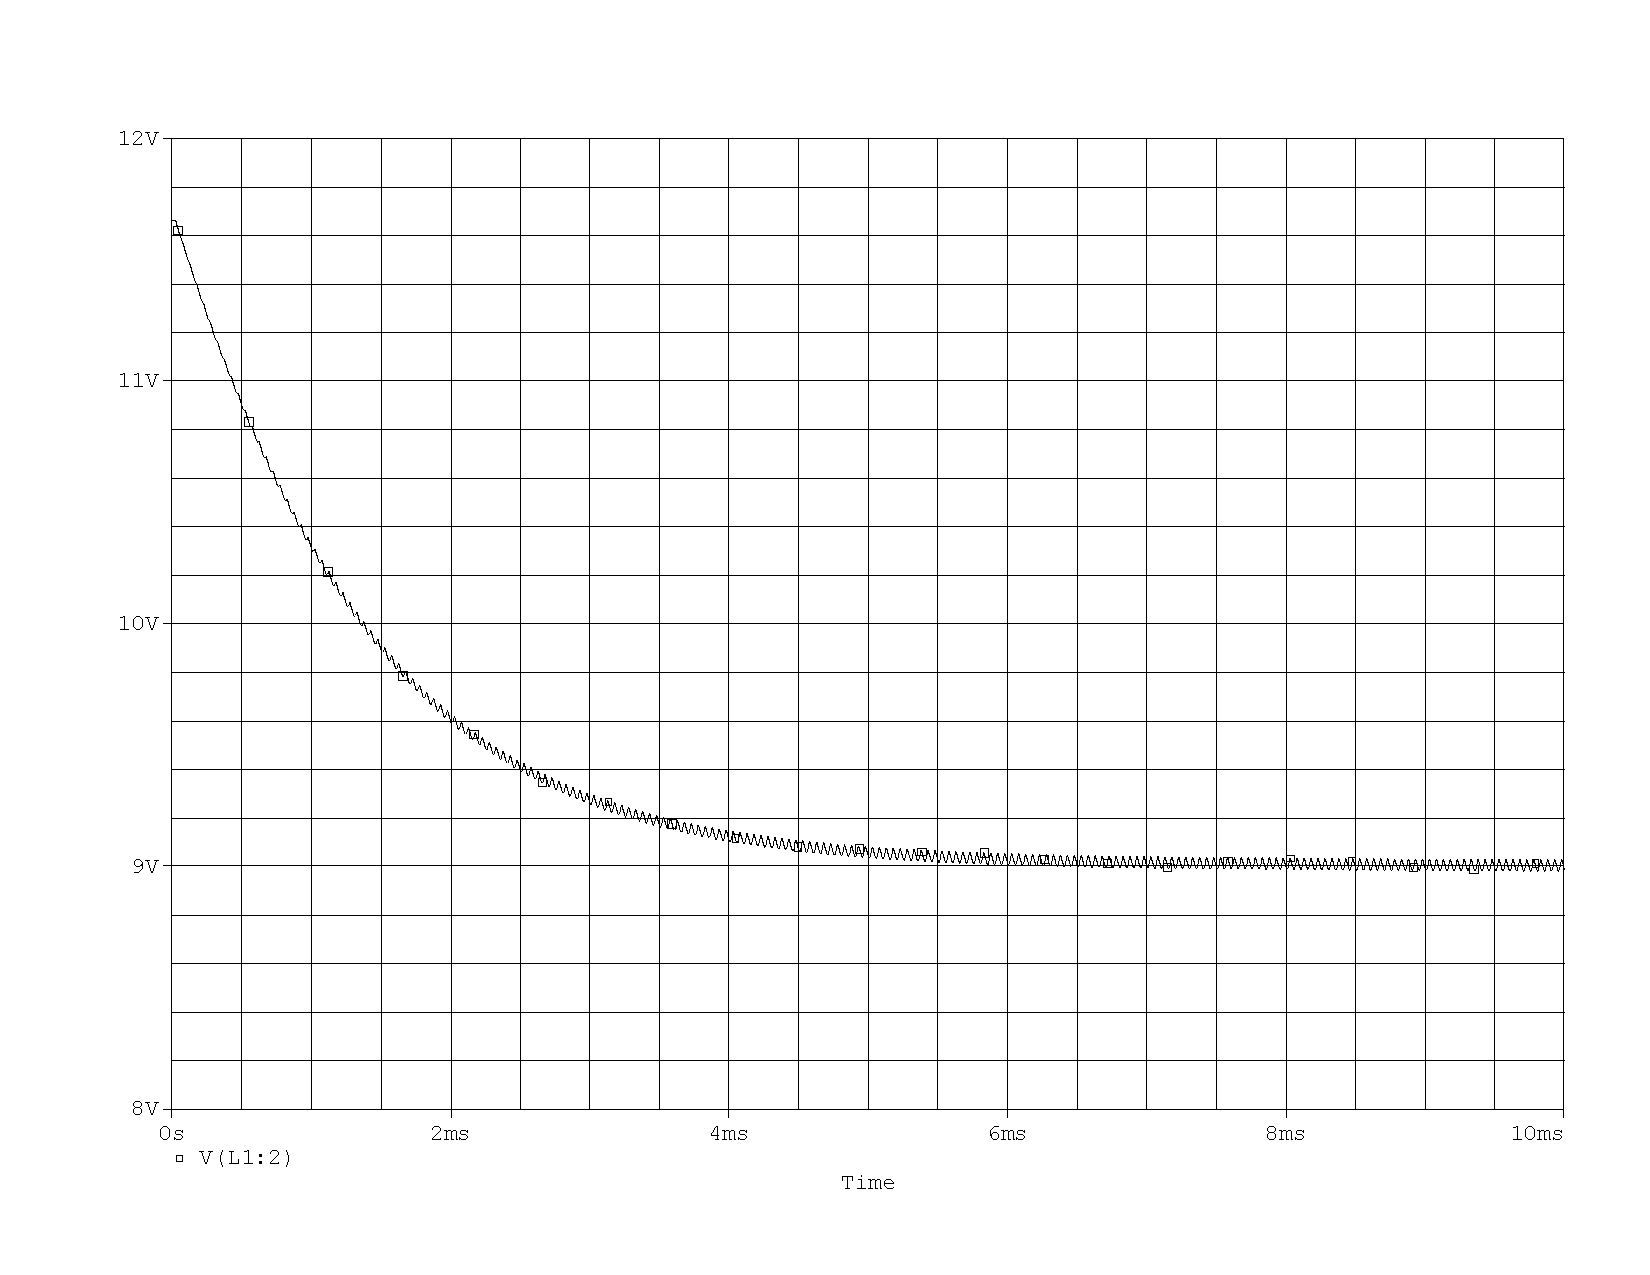
\includegraphics[scale=0.5]{Figuras/ej1_vo.pdf}
	\caption{Tensión de salida.}
	\label{fig:sim_ej1_vo}
\end{figure}

\begin{figure}[H]
	\centering
	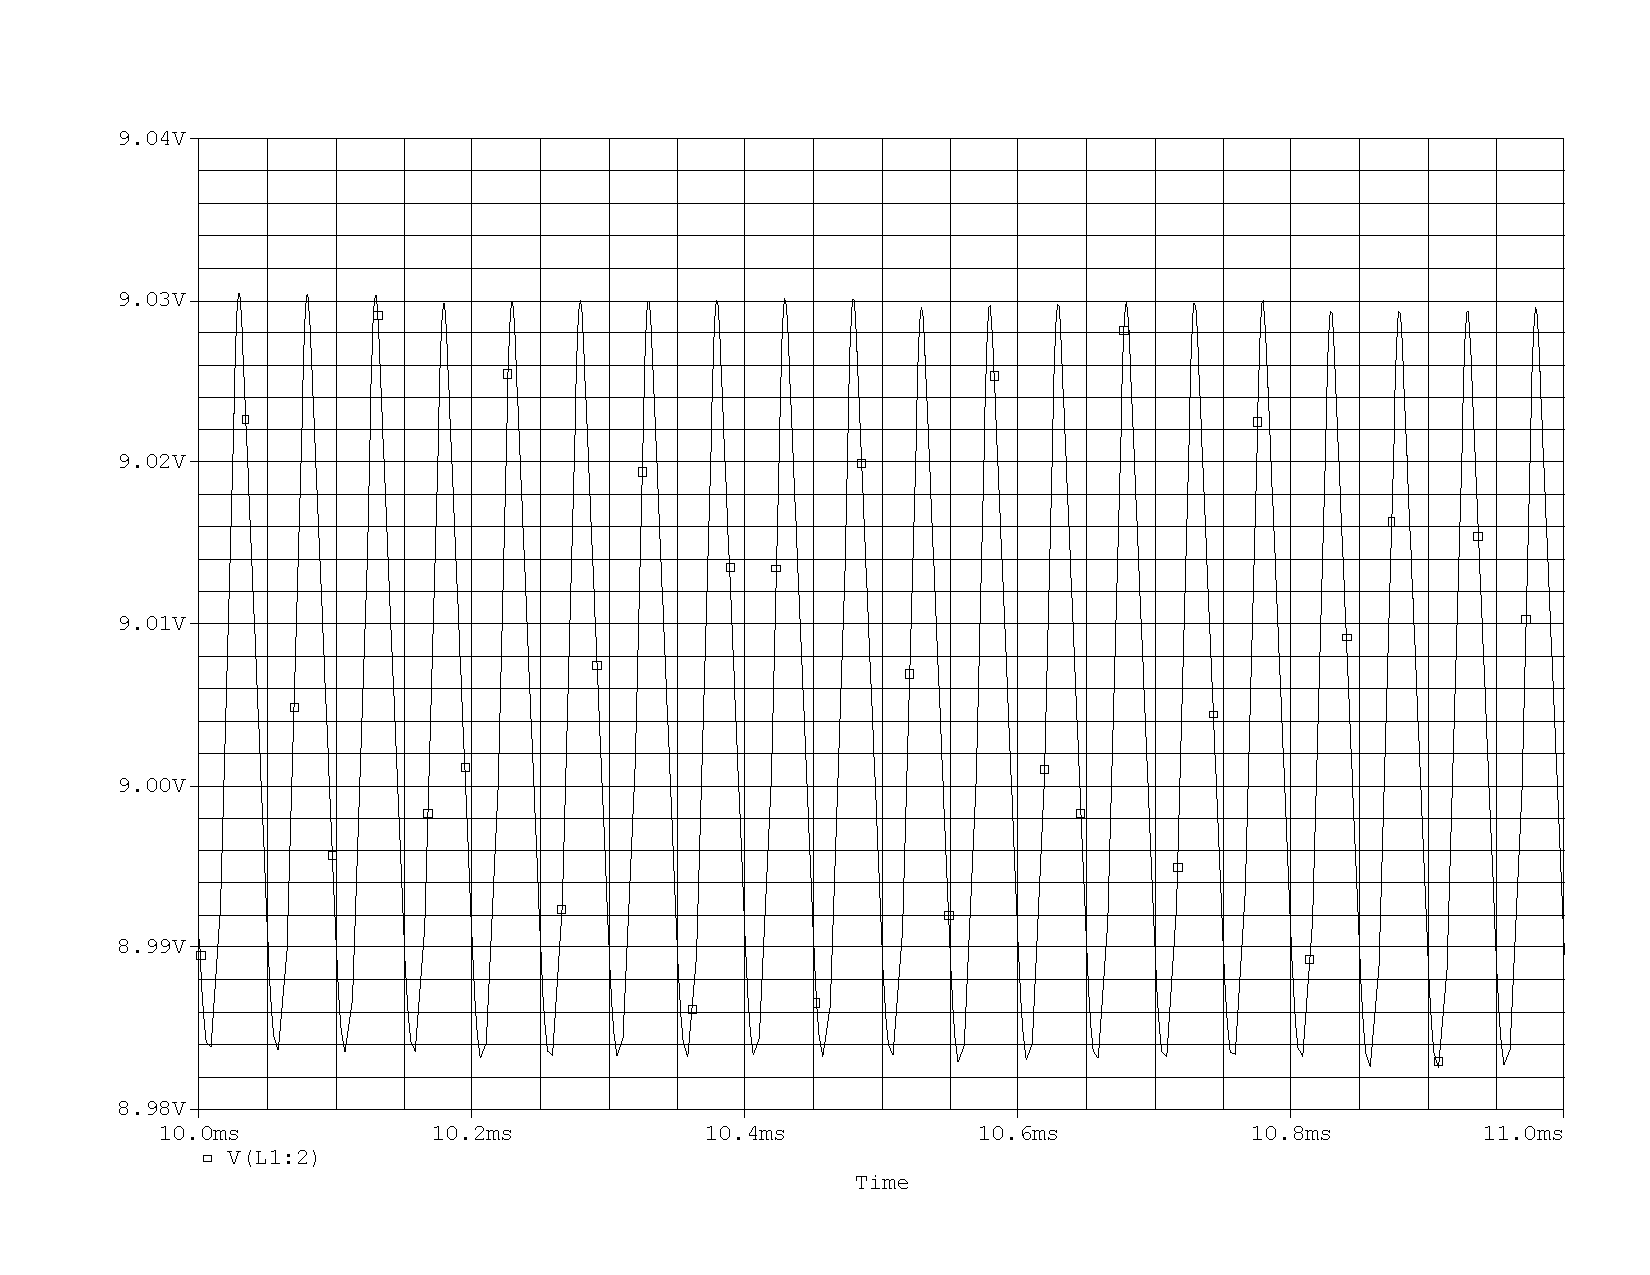
\includegraphics[scale=0.5]{Figuras/ej1_vo_zoom.pdf}
	\caption{Tensión de salida.}
	\label{fig:sim_ej1_vo_zoom}
\end{figure}

\Flor{Ripple da \SI{46.5}{\milli\volt} }

\begin{figure}[H]
	\centering
	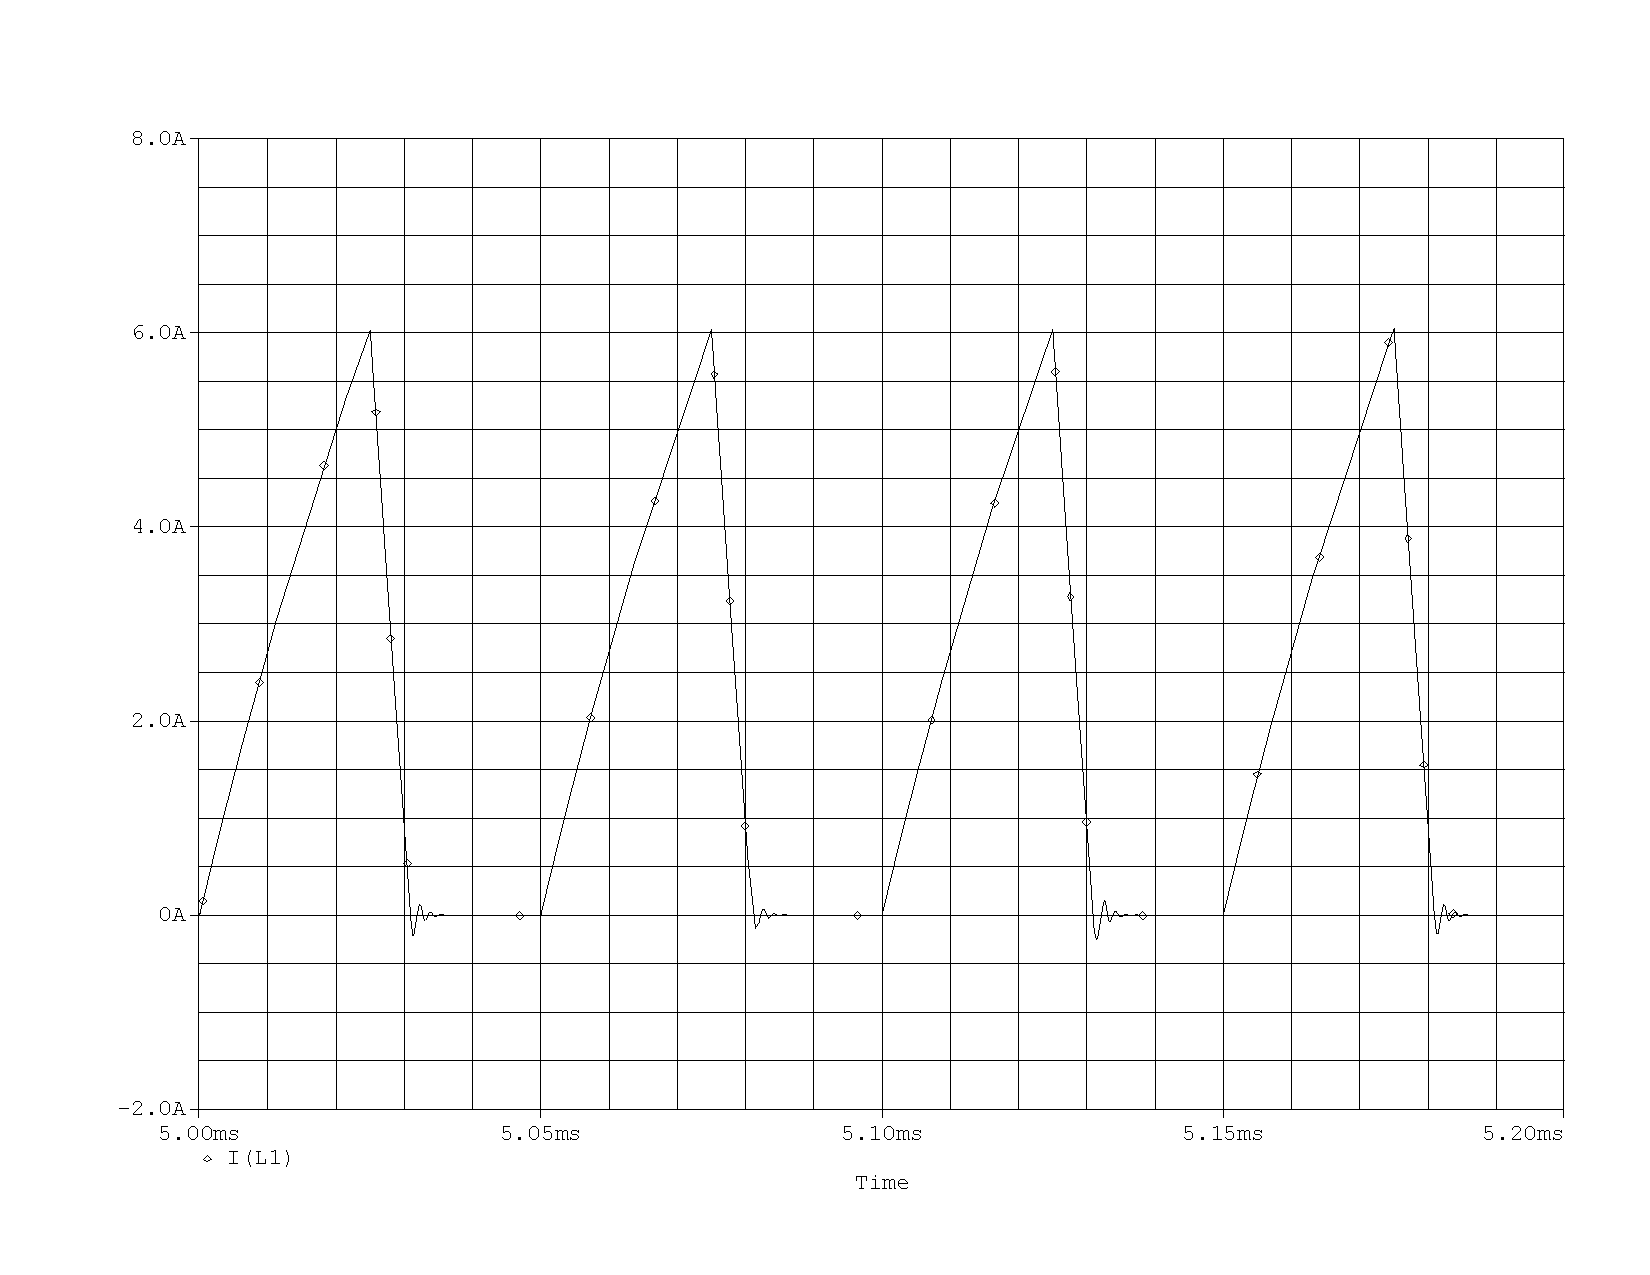
\includegraphics[scale=0.5]{Figuras/ej1_I(L1).pdf}
	\caption{Corriente en el inductor.}
	\label{fig:sim_ej1_vo}
\end{figure}


		
	\part{Ejercicio 2}\label{part:ej2}
		\section{Análisis teórico}\label{sec:teo2}
			\begin{figure}[H]
	\centering
	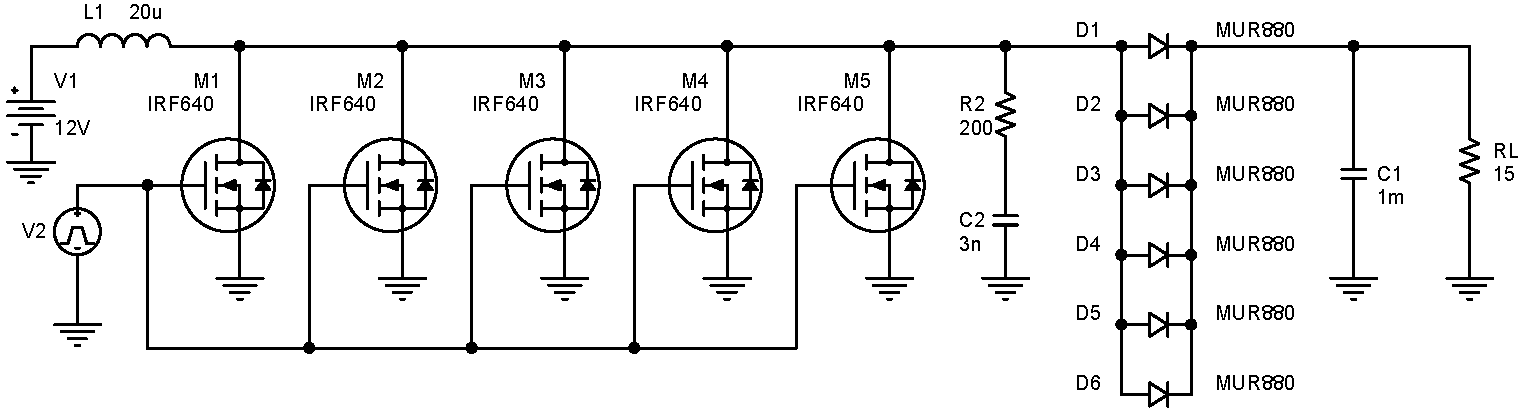
\includegraphics[scale=0.3]{Circ2}
	\caption{Circuito completo.}.
	\label{fig:Circ2}
\end{figure}


El circuito del Esquema \ref{fig:Circ2} corresponde a un regulador \textit{Flyback}. Su funcionamiento puede analizarse en dos ciclos. 

\begin{itemize}
	\item \textbf{Primer ciclo:} cuando la señal de pulso toma el valor de \SI{12}{\volt}, $V_{GS}=\SI{12}{\volt}$ por lo que el MOSFET está en conducción. El diodo $D$ se encuentra polarizado en inversa y la corriente que circula por el inductor produce almacenamiento de energía en su núcleo. El circuito simplificado se representa en la Figura \ref{fig:1ciclo}.

		Es posible calcular la corriente en el inductor máxima, sabiendo que el pulso tiene una frecuencia de \SI{20}{\kilo\hertz} y que posee medio ciclo de trabajo.

		\begin{equation}
			\centering
			I_{L1}(t) = \frac{V_1}{R_{DS<on>}} \left(1-\exp{(-t/\tau)}\right),
		\end{equation}
		siendo $t_{carga} = \tau=L1/R_{DS<on>} = \SI{533}{\micro\second}$. El periodo del pulso es $\SI{50}{\micro\second} < t_{carga}$
entonces la corriente máxima en el inductor es

		\begin{equation}
			\centering
					I_{L1}(\SI{25}{\micro\second}) = \frac{\SI{12}{\volt}}{\SI{0.0375}{\ohm} } \left(1-\exp{(\SI{-25}{\micro\second}/ \SI{533}{\micro\second})}\right) = \SI{14.7}{\ampere}
		\end{equation}

	
\HgraficarEPS{0.5}{cto_ej2_1ciclo}{Primer ciclo}{fig:1ciclo}


\item \textbf{Segundo ciclo:}
	Cuando el pulso vale \SI{0}{\volt}, el MOSFET se encuentra en corte, lo cual equivale a una impedancia muy elevada. Debido a que la corriente en el inductor no puede cambiar instantáneamente, se invierte la polaridad de la tensión en el inductor y el diodo pasa a estar en directa. Se produce una transferencia de energía desde el inductor al capacitor hasta que el inductor se descargue por completo. Debido a que la tensión en el inductor se invierte (\textit{flies back}), la tensión en la salida es mayor que la de entrada. El circuito simplificado se muestra en la Fiugra \ref{fig:2ciclo}.

\HgraficarEPS{0.5}{cto_ej2_2ciclo}{Segundo ciclo}{fig:2ciclo}

		El regulador opera en modo discontinuo, por lo que el inductor se descarga completamente en cada ciclo, es decir que la corriente en el inductor se anula. El comportamiento de la corriente en el inductor se ilustra en la Figura \ref{fig:mod_dis}. El tiempo de descarga debe ser menor al de carga. $T > t_{carga} + t_{descarga}$, considerando $t_{descarga} = \SI{10}{\micro\second}$, el valor de $D$ (\textit{duty cycle}) es 

		\begin{equation}
			\centering
			D = \frac{t_{carga}}{t_{carga} + t_{descarga}} \cong \boxed{\num{0,7}}
		\end{equation}
		
	%	\Flor{Encontré esta fórmula, que es parecida a (17)}
	%	La tensión de salida puede aproximarse

	%	\begin{equation}
	%		\centering
	%		V_S \cong V_E \left( 1 + \frac{t_{carga}}{t_{descarga}} \right) = \SI{12}{\volt} \left(1+ \frac{25}{15}\right) = \boxed{\SI{32}{\volt}}
	%	\end{equation}
\end{itemize}


\HgraficarEPS{0.6}{modo_discontinuo}{Modo discontinuo}{fig:mod_dis}


%\Gus{Tiro ecuaciones que seguro se van a usar, al menos son las que use para intentar el calculo}
%\Flor{Creo que estas ecuaciones no se usan}
%
%\begin{equation}
%	{L} = \frac{(1-D) \cdot (V_s - V_E)}{2 \cdot f \cdot (I_{L_{max}} - I_{L_{prom}})}
%\end{equation}
%
%\Gus{verificar esta ecuacion}
%\begin{equation}
%	V_s = \frac{(V_E - V_{sat})}{1-D} - V_D \cdot (1 - D) 
%	\label{ec:Nose}
%\end{equation}
%
%\Flor{En la diapo está un toque distinta}
%
%\textcolor{blue}{$$V_S = (V_E-V_{SAT}) \left(  1 + \frac{t_{carga}}{t_{descarga}} \right) -V_D$$}
%
%\Gus{Grafico XX de $I_S$ respecto al tiempo tengo que sacarlo de las diapos}

La corriente de salida está dada por \eqref{ec:is}.
\begin{equation}
	I_s = \frac{I_{max} \cdot (1-D) \cdot T}{2 \cdot T} = \frac{I_{max} \cdot (1 - D)}{2} 
	\label{ec:is}
\end{equation}

Al estar trabajando en modo discontinuo se cumple que $ 2 I_{L_{prom}} =I_{L_{max}} $ por lo tanto.


\begin{equation}
	L = \frac{(1 - D)^2 \cdot (V_s - V_E)}{2 \cdot f \cdot (I_s)}
\end{equation}

Despejando y tomando a $\frac{V_s}{I_s} = R_L = \SI{15}{\ohm}$


\begin{equation}
	I_s^{-1} = \frac{\SI{15}{\ohm} - \frac{L \cdot 2 \cdot f}{(1-D)^2}}{V_E}
\end{equation}

Con $D=0,7$

\begin{equation}
	\boxed{I_s = \SI{1,963}{\ampere}}
\end{equation}


\begin{equation}
	\boxed{V_s = R_L \cdot I_s = \SI{29,45}{\volt}}
\end{equation}



		\section{Simulaciones}\label{sec:sim2}
			\begin{figure}[H]
	\centering
	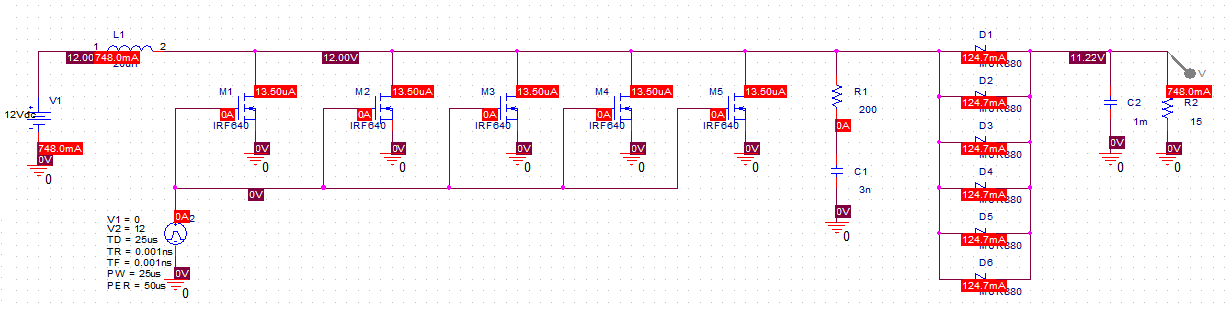
\includegraphics[scale=0.4]{ej2_esq_sim}
	\caption{Simulación en \textit{PSpice}.}
	\label{fig:ej2_esq_sim}
\end{figure}

Se simuló el circuito \ref{fig:ej2_esq_sim}, y se obtuvo la tensión de salida según se ilustra en la Figura \ref{fig:ej2_vo}, aunque posee una pendiente, se puede aproximar $V_S \cong \SI{31}{\volt}$, valor similar al obtenido analíticamente.

\begin{figure}[H]
	\centering
	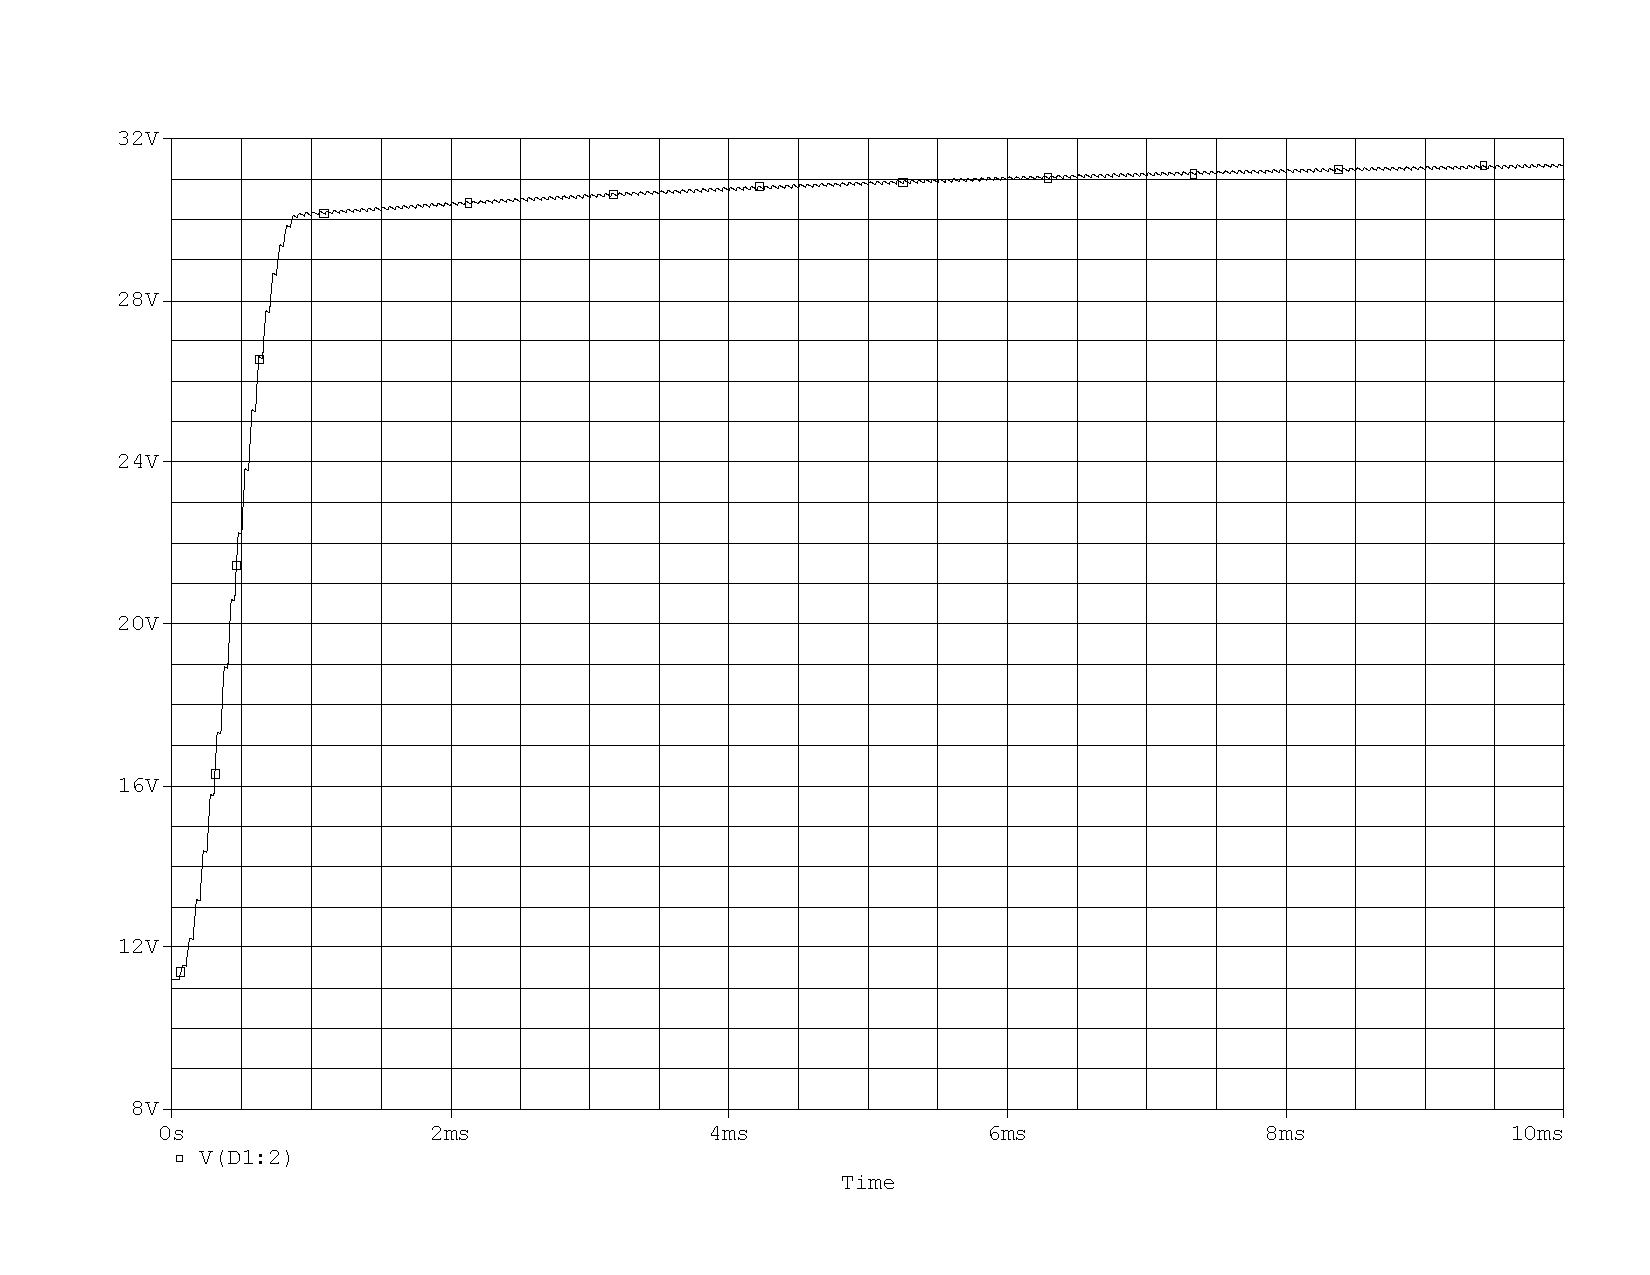
\includegraphics[scale=0.4]{ej2_vo.pdf}
	\caption{Tensión de salida.}
	\label{fig:ej2_vo}
\end{figure}


\begin{figure}[H]
	\centering
	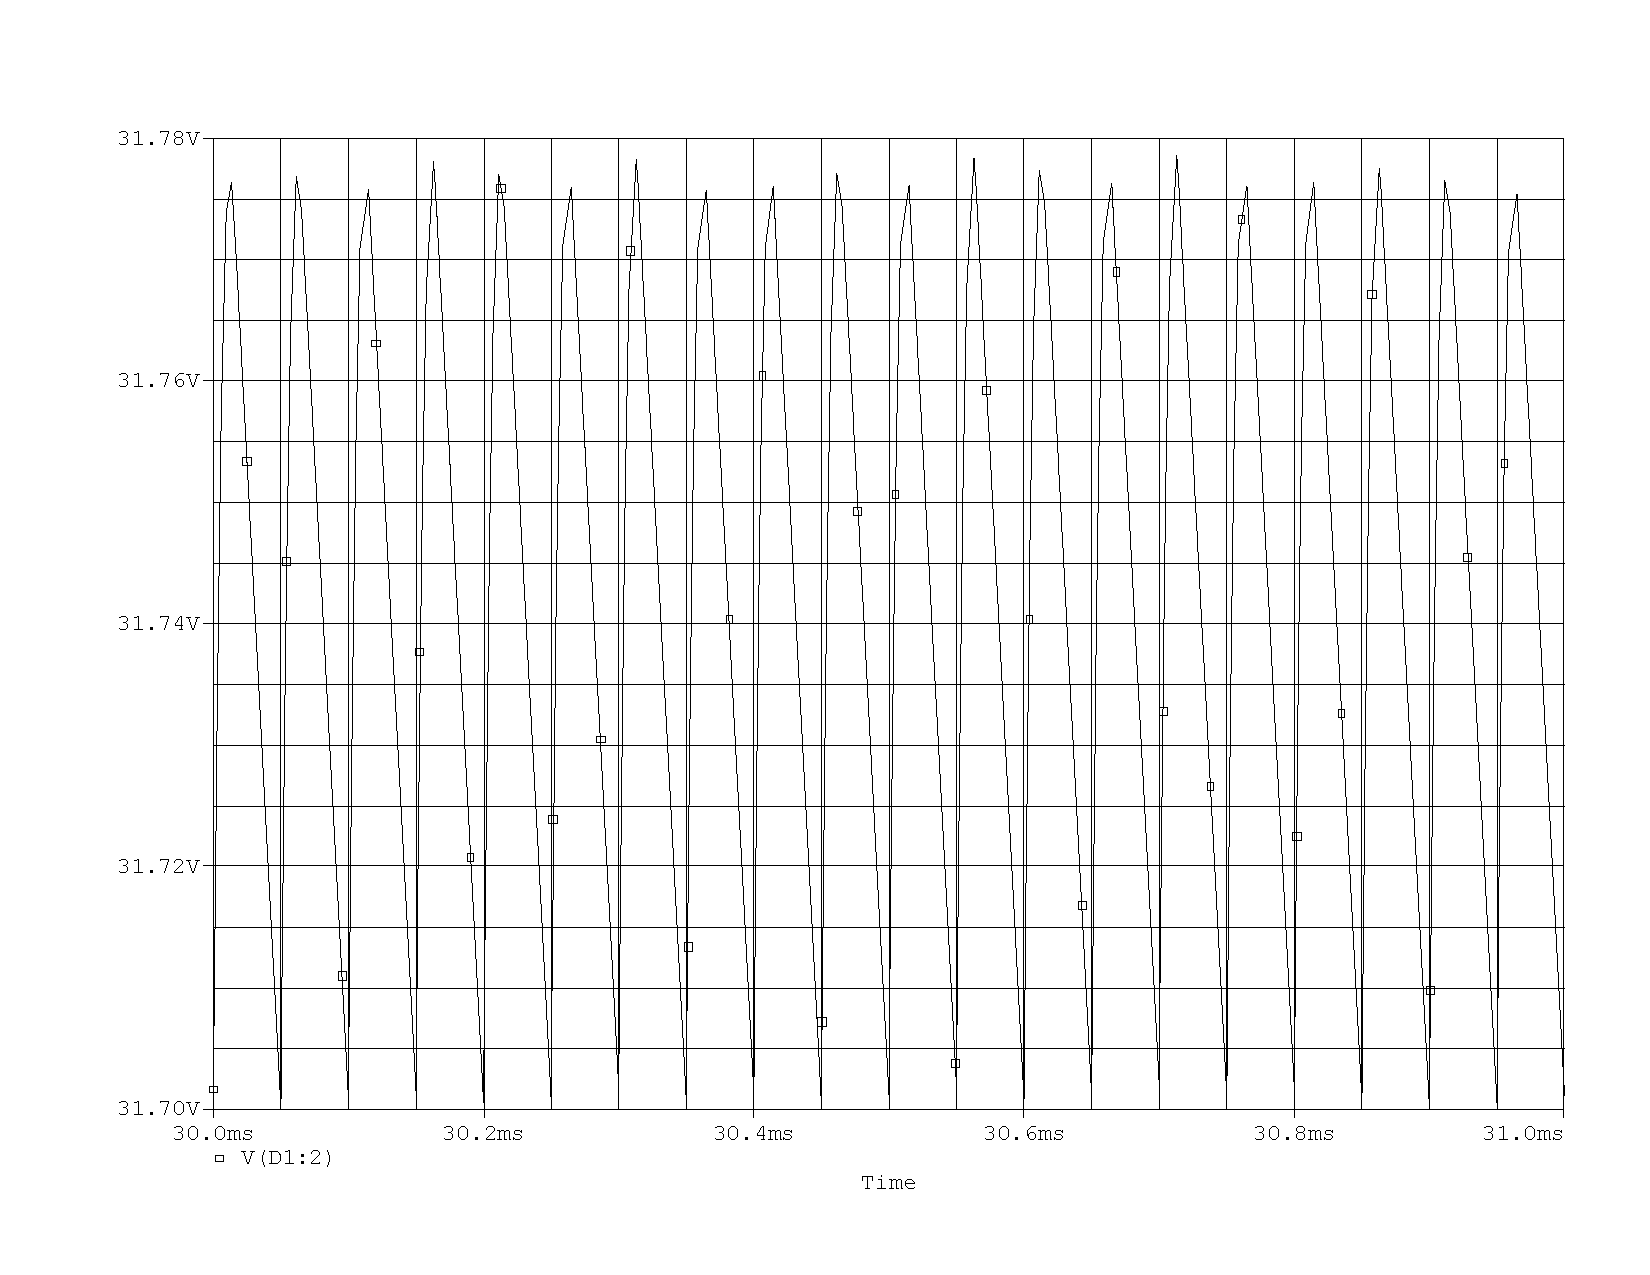
\includegraphics[scale=0.4]{ej2_vo_zoom.pdf}
	\caption{Tensión de salida.}
	\label{fig:ej2_vo_zoom}
\end{figure}

A su vez al ampliar la curva de salida \ref{fig:ej2_vo_zoom} se observa que no es una recta, sino que presenta un rizado de valor \eqref{ec:riz2}.

\begin{equation}
	\centering
	\Delta V_o = \SI{31.775}{\volt} - \SI{31.7}{\volt} = \boxed{\SI{75}{\milli\volt}}
	\label{ec:riz2}
\end{equation}

\begin{figure}[H]
	\centering
	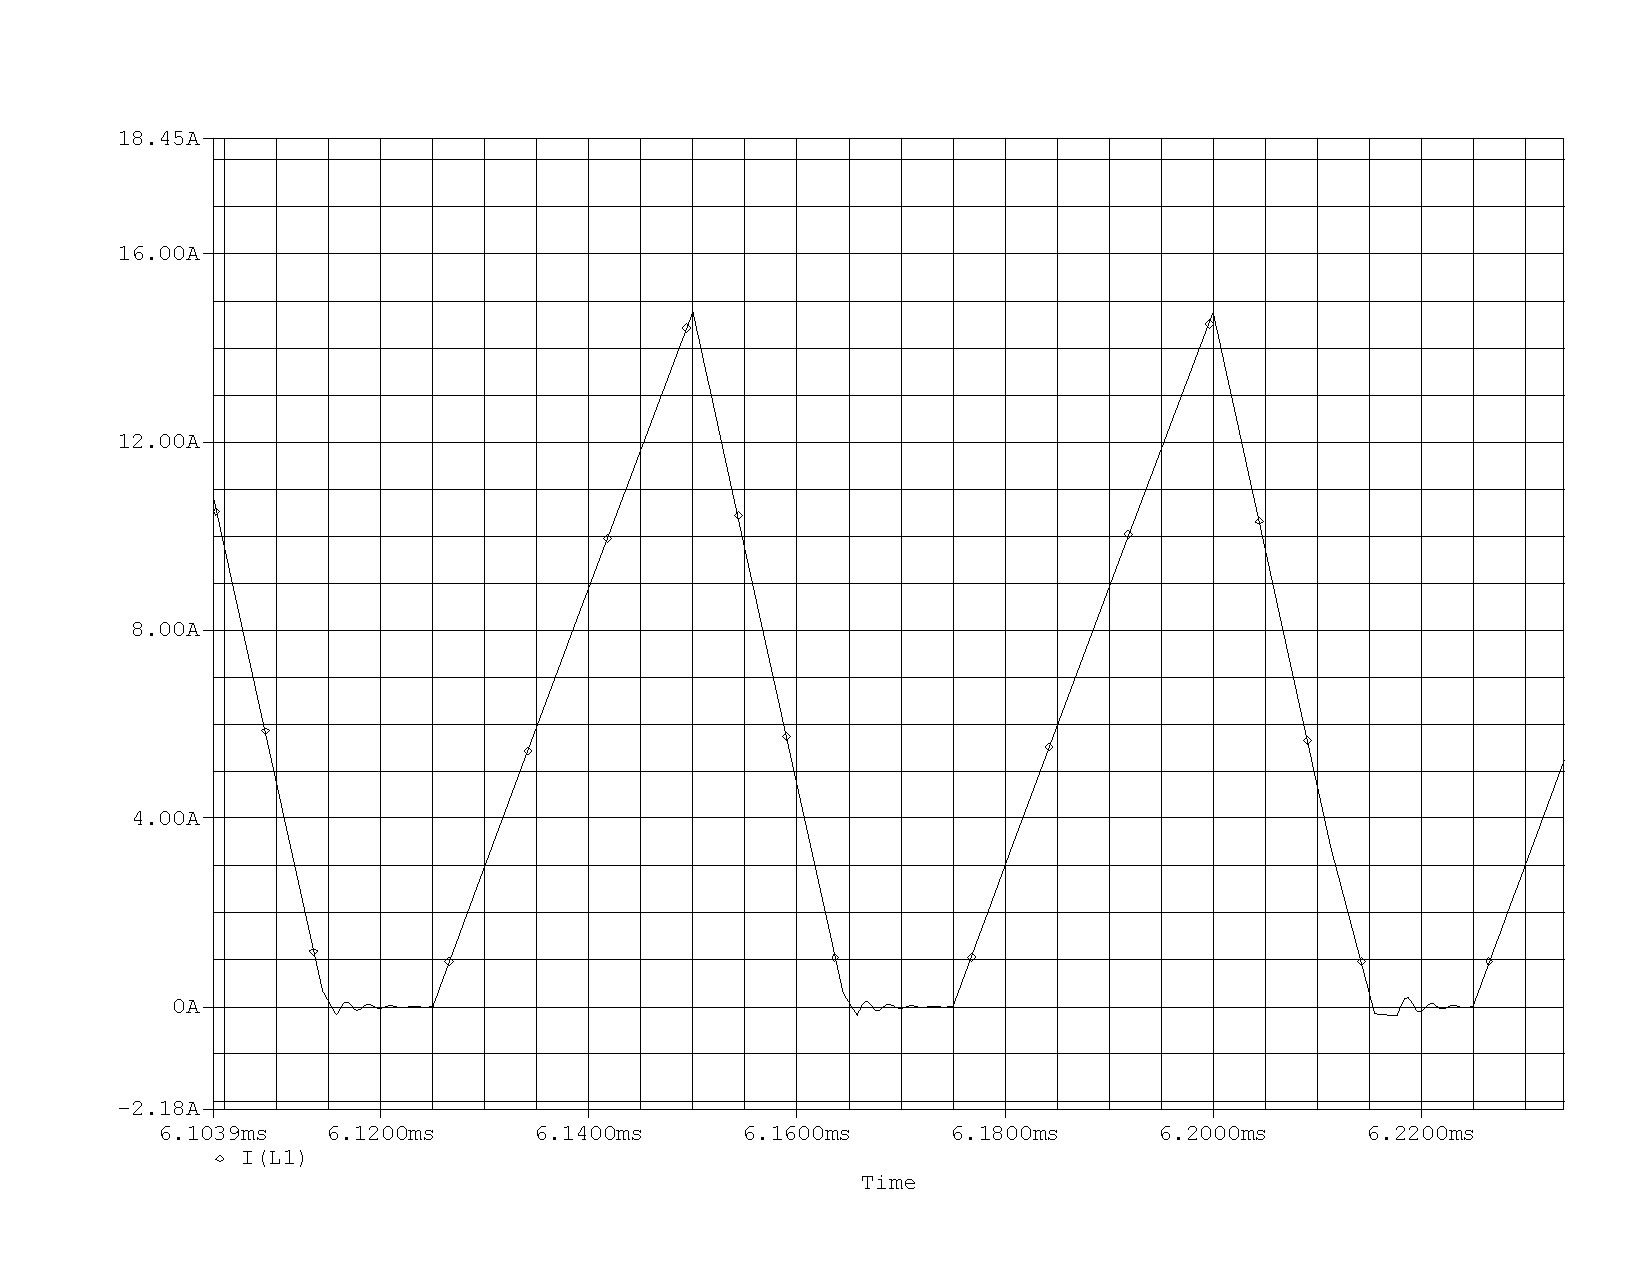
\includegraphics[scale=0.4]{ej2_i_L1.pdf}
	\caption{Corriente en el inductor.}
	\label{fig:ej2_i_L1}
\end{figure}


A partir de la Figura \ref{fig:ej2_i_L1} se verifica el funciomiento del circuito en modo discontinuo, siendo la corriente máxima \SI{14.7}{\ampere} coincidente con la hallada analíticamente. Asimismo se corrobora que el tiempo de carga es mayor que el de descarga, siendo sus valores semejantes a los obtenidos teóricamente.


		
	\part{Conclusiones}\label{part:conclusiones}
		La principal diferencia entre los dos circuitos estudiados radica en la tensión de salida, en el primer caso siempre se cumple $V_S < V_E$, mientras que en el segundo circuito la tensión de salida siempre superará a la de entrada.
Otro parámetro importante a tener en cuenta es la tensión de rizado en la salida. En el primer caso se obtuvo un menor rizado que en el segundo. 

Por otra parte, se observa que ambos presentan transistores y diodos en paralelo. Esto permite obtener una mejor distribución de la corriente, haciendo que cada dispositivo maneje menos corriente y por ende menor caída de tensión en él.

Asimismo, poseen una red $RC$ denominada \textit{snub} en paralelo al diodo para el primer regulador y en paralelo al arreglo de transistores en el regulador \textit{Flyback}. La función del \textit{snub} es amortiguar la sobretensión que ocurre en el inductor ante las conmutaciones, evitando la destrucción de los dispositivos.



	% \appendix
\end{document}
